\chapter{Ramsey Theory}

\section{Introduction to Ramsey Theory}

``Complete Disorder is impossible''

% 8.1
\topic{The party problem}
Imagine you want to plan a party and you want to avoid that a few guests only will end up alone. You want to know how many guests you will have to invite such that either $m$ many mutually know each other or $n$-many are mutual strangers. We will see that this will always happen eventually. That number is called the Ramsey number $R(m,n)$.

% 8.2
\topic{History}
\begin{itemize}
    \item Area based on a paper by Frank Ramsey ``On a problem of formal logic'' (1928).
    \item Ramsey (1903--1930), although dying very young, contributed to many different areas of research -- Economy (Ramsey pricing), philosophy (Ramsey sentences), Logic (Ramsey expansions) and mathematics (Ramsey numbers).
\end{itemize}

% 8.3 Definition
\begin{definition}
Let $G$ be a graph. An \textbf{\color{red}edge $k$-colouring} of $G$ is any function $K: E_G \to \{1, 2, \dots, k\}$. 
\end{definition}
In this course, we will mainly consider 2-colourings of edges and set the colours to be $\{red, green\}$.\\
Note that there are no conditions on the function except for the domain and codomain.

% 8.4 Example
\begin{example}
Consider the following edge colourings of $K_5$.
\begin{center}
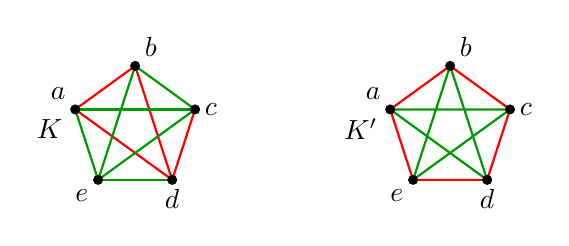
\begin{tikzpicture}[scale=0.8]
    % Left K5 (K)
    \begin{scope}[xshift=0cm]
        \node[left] at (-1,0) {$K$};
        \foreach \i in {1,...,5} \coordinate (v\i) at (90+72*\i:1);
        
        % Edges (Red triangle a,b,d -> v1, v5, v3)
        % Labels in notes: a=top left, b=top right, c=right, d=bottom right, e=bottom left?
        % Let's match visual shape.
        % a (v1), b (v5), c (v4), d (v3), e (v2) based on star shape.
        
        \coordinate (a) at (v1); \node[above left] at (a) {$a$};
        \coordinate (b) at (v5); \node[above right] at (b) {$b$};
        \coordinate (c) at (v4); \node[right] at (c) {$c$};
        \coordinate (d) at (v3); \node[below] at (d) {$d$};
        \coordinate (e) at (v2); \node[below left] at (e) {$e$};
        
        % Red triangle a,b,d
        \draw[red, thick] (a)--(b);
        \draw[red, thick] (b)--(d);
        \draw[red, thick] (a)--(d);
        \draw[red, thick] (c)--(d);
        
        % Other edges (Green)
        \draw[green!60!black, thick] (a)--(c);
        \draw[green!60!black, thick] (a)--(e);
        \draw[green!60!black, thick] (b)--(c);
        \draw[green!60!black, thick] (b)--(e);
        \draw[green!60!black, thick] (c)--(e);
        \draw[green!60!black, thick] (d)--(e);
        
        \foreach \p in {a,b,c,d,e} \filldraw (\p) circle (2pt);
    \end{scope}

    % Right K5 (K')
    \begin{scope}[xshift=5cm]
        \node[left] at (-1,0) {$K'$};
        \foreach \i in {1,...,5} \coordinate (u\i) at (90+72*\i:1);
        \coordinate (a) at (u1); \node[above left] at (a) {$a$};
        \coordinate (b) at (u5); \node[above right] at (b) {$b$};
        \coordinate (c) at (u4); \node[right] at (c) {$c$};
        \coordinate (d) at (u3); \node[below] at (d) {$d$};
        \coordinate (e) at (u2); \node[below left] at (e) {$e$};
        
        % Approximate the second graph (Pentagon green, star red)
        \draw[green!60!black, thick] (u1)--(u3)--(u5)--(u2)--(u4)--(u1);
        \draw[red, thick] (u1)--(u2)--(u3)--(u4)--(u5)--(u1);
        
        \foreach \i in {1,...,5} \filldraw (u\i) circle (2pt);
    \end{scope}
\end{tikzpicture}
\end{center}
Note that $K$ produced a triangle on $\{a,b,d\}$ whose edges are all red, whereas with $K'$ there is neither a red nor a green triangle.
\end{example}

% 8.5 Definition
\begin{definition}
\begin{enumerate}
    \item[1)] Let $G$ be a graph and $K: E_G \to \{1, \dots, k\}$ an edge colouring. We call a subgraph $H \subseteq G$ \textbf{\color{red}monochromatic} if all edges of $H$ have the same colour, i.e. $K|_H : E_H \to \{1, \dots, k\}$ has a range of size 1, $|K(E_H)|=|\{i\}|=1$. We then call $H$ a graph of colour $i$.
    \item[2)] The \textbf{\color{red}Ramsey number $R(a,b)$} for $a,b \in \mathbb{Z}_+$ is the smallest integer $n$ s.t. any edge 2-colouring of $K_n$ either contains a red $K_a$ or a green $K_b$ as a subgraph.
\end{enumerate}
\end{definition}

% 8.6 Example
\begin{example}
\begin{enumerate}
    \item[1)] First note that $R(a,b) = R(b,a)$ for all $a,b \in \mathbb{Z}_+$. (Exercise)
    \item[2)] Let's observe $R(1,b)$ is the least $n \in \mathbb{Z}_+$ s.t. any edge 2-colouring contains either a red $K_1$ or a green $K_b$. As $K_1$ does not contain any edges, every edge colouring of any non-empty graph satisfies the condition, whence $R(1,b)=1$.
    \item[3)] $R(2,2)=2$, as any edge 2-colouring of $K_2$ either colours the unique edge red or green, whence we either obtain a red or green $K_2$.
\end{enumerate}
\end{example}

% 8.7 Lemma
\begin{lemma}
Let $r \ge R(a,b)$ for $a,b \in \mathbb{Z}_+$. Then any edge 2-colouring of $K_r$ produces either a red $K_a$ or a green $K_b$.
\end{lemma}

\begin{proof}
Let $k := R(a,b)$, $r \ge k$ and $K$ be any edge 2-colouring of $K_r$. Clearly, $K_r$ contains $K_k$ as a subgraph. Then $K_k$, and hence $K_r$, either contains a red $K_a$ or a green $K_b$, as desired.
\end{proof}

% 8.8 Lemma
\begin{lemma}
We have that $R(3,4) = 9$.
\end{lemma}

\begin{proof}
We have to show two things: 1) $R(3,4) > 8$ and 2) $R(3,4) \le 9$.

1) $R(3,4) > 8$, i.e. exists an edge 2-colouring of $K_8$ without a red $K_3$ and green $K_4$:
\begin{center}
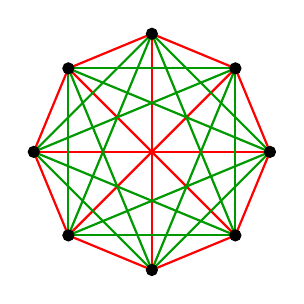
\begin{tikzpicture}[scale=1]
    % K8 layout
    \foreach \i in {1,...,8} \coordinate (v\i) at (90+45-45*\i:1.5);
    
    % Draw "Wagner graph" style / specific Ramsey coloring for K8 (3,4) lower bound
    % Outer cycle + chords of length 1, 4 (Red)
    % Edges connecting i to i+1 and i to i+4 are RED
    \foreach \i [evaluate=\i as \j using {int(mod(\i,8)+1)}] in {1,...,8} \draw[red, thick] (v\i)--(v\j);
    \draw[red, thick] (v1)--(v5); \draw[red, thick] (v2)--(v6); 
    \draw[red, thick] (v3)--(v7); \draw[red, thick] (v4)--(v8);
    
    % All other edges GREEN
    % Distance 2 and 3 chords
    \foreach \i [evaluate=\i as \j using {int(mod(\i+1,8)+1)}] in {1,...,8} \draw[green!60!black, thick] (v\i)--(v\j);
    \foreach \i [evaluate=\i as \j using {int(mod(\i+2,8)+1)}] in {1,...,8} \draw[green!60!black, thick] (v\i)--(v\j);
    
    % Draw nodes
    \foreach \i in {1,...,8} \filldraw (v\i) circle (2pt);
\end{tikzpicture}
\end{center}

2) $R(3,4) \le 9$, i.e. any edge 2-colouring of $K_9$ either produces a red $K_3$ or a green $K_4$.
\underline{Claim:} There is a vertex $v$ with either at least 4 red or at least 6 green edges incident.
$\hookrightarrow$ Otherwise, as all vertices have degree 8, all vertices must be incident with exactly 3 red and 5 green edges. Consider then the subgraph $H \subseteq G$ consisting of all 9 vertices of $G$ and all red edges. Then $H$ is a graph which has odd many (i.e. 9) vertices of odd (i.e. 3) degree, contradicting the Handshaking Lemma.

$\blacktriangleright$ Now consider first the case that ex. $v \in V_G$ incident with 4 red edges, say $\{vx_1, vx_2, vx_3, vx_4\}$. If any of the edges $x_ix_j$ is also red, we have a red $K_3$ on $\{v, x_i, x_j\}$. Otherwise, all these edges are blue [green] and we get a blue [green] $K_4$ on $\{x_1, x_2, x_3, x_4\}$, as desired.

\begin{center}
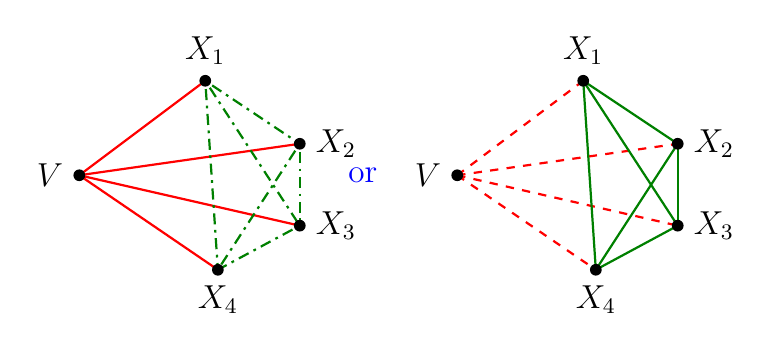
\begin{tikzpicture}[
    scale=0.8,
    node_style/.style={circle, fill=black, inner sep=1.5pt},
    label_style/.style={font=\sffamily\large},
    red_solid/.style={red, thick},
    red_dashed/.style={red, thick, dashed},
    green_solid/.style={green!50!black, thick},
    green_dotted/.style={green!50!black, thick, dash pattern=on 1pt off 2pt on 4pt off 2pt} % loose dash-dot look
]

    % --- Define coordinates for the relative shape ---
    % We define them once relative to (0,0) then shift for the second graph
    \def\drawgraph#1#2{
        % #1: Red style, #2: Green style
        
        \coordinate (V) at (0,0);
        \coordinate (X1) at (2, 1.5);
        \coordinate (X2) at (3.5, 0.5);
        \coordinate (X3) at (3.5, -0.8);
        \coordinate (X4) at (2.2, -1.5);

        % Draw Edges V -> Xs (Red)
        \draw[#1] (V) -- (X1);
        \draw[#1] (V) -- (X2);
        \draw[#1] (V) -- (X3);
        \draw[#1] (V) -- (X4);

        % Draw Edges X <-> X (Green)
        \draw[#2] (X1) -- (X2);
        \draw[#2] (X1) -- (X3);
        \draw[#2] (X1) -- (X4);
        \draw[#2] (X2) -- (X3);
        \draw[#2] (X2) -- (X4);
        \draw[#2] (X3) -- (X4);

        % Draw Nodes
        \node[node_style, label=left:{\large $V$}] at (V) {};
        \node[node_style, label=above:{\large $X_1$}] at (X1) {};
        \node[node_style, label=right:{\large $X_2$}] at (X2) {};
        \node[node_style, label=right:{\large $X_3$}] at (X3) {};
        \node[node_style, label=below:{\large $X_4$}] at (X4) {};
    }

    % --- LEFT GRAPH ---
    % Red Solid, Green Dotted
    \drawgraph{red_solid}{green_dotted}

    % --- MIDDLE TEXT ---
    \node[blue, font=\large] at (4.5, 0) {or};

    % --- RIGHT GRAPH ---
    % Shift to the right
    \begin{scope}[xshift=6cm]
        % Red Dashed, Green Solid
        \drawgraph{red_dashed}{green_solid}
    \end{scope}

\end{tikzpicture}
\end{center}

$\blacktriangleright$ Now, in the leftover case, $v$ has six green incident edges. Say $\{vx_1, \dots, vx_6\}$. As $R(3,3)=6$ (HW), we get that there is either a red $K_3$ contained in $\langle \{x_1, \dots, x_6\} \rangle$, in which case we are done, or a green $K_3$, say on $\{x_i, x_j, x_k\}$. But then we find a green $K_4$ on $\{v, x_i, x_j, x_k\}$ and again our claim holds.

We thus saw that there is a 2-colouring of the edges of $K_8$ without a red $K_3$ or green $K_5$, however every 2-colouring of the edges of $K_9$ produces either a red $K_3$ or a green $K_4$. Thus, $R(3,4)=9$.
\end{proof}

% 8.9 Summary
\topic{Summary and more...}
Let us sum up some of the known Ramsey numbers.
\begin{center}
\renewcommand{\arraystretch}{1.5}
\begin{tabular}{c|c|c}
$a$ & $b$ & $R(a,b)$ \\
\hline
1 & $k$ & 1 \\
2 & $k$ & $k$ \\
3 & 3 & 6 \\
3 & 4 & 9 \\
3 & 5 & 14 \\
3 & 6 & 18 \\
\end{tabular}
\hspace{1cm}
\begin{tabular}{c|c|c}
$a$ & $b$ & $R(a,b)$ \\
\hline
3 & 7 & 23 \\
3 & 8 & 28 \\
3 & 9 & 36 \\
4 & 4 & 18 \\
4 & 5 & 25 \\
5 & 5 & $????$
\end{tabular}
\end{center}
The problem gets very fast very complicated. Why should there even always be an answer?

% 8.10 Theorem
\begin{theorem}[Ramsey]
For any positive integers $a,b$ the Ramsey number $R(a,b)$ exists, i.e. there is a positive integer $n$ s.t. every edge 2-colouring of $K_n$ either produces a red $K_a$ or a green $K_b$.
\end{theorem}

\begin{proof}
We establish the proof by induction on $m := a+b$.
\underline{$m=2$}: If $a+b=2$, then $a=b=1$ and we know that $R(1,1)=1$.

\underline{$m \to m+1$}: Assume for any $\tilde{a}, \tilde{b} \in \mathbb{Z}_+$ with $\tilde{a}+\tilde{b} \le m$ we know that $R(\tilde{a}, \tilde{b})$ exists. Now assume $a,b \in \mathbb{Z}_+$ s.t. $a+b=m+1$. Then both $R(a-1, b)$ and $R(a, b-1)$ exist by I.H. Set $n := R(a-1, b) + R(a, b-1)$ and consider $K_n$. We claim that $K_n$ does the job.
To this end, pick an arbitrary edge 2-colouring $K$ of $K_n$ and choose $v \in V(K_n)$ arbitrary. Define two sets:
\[ A := \{w \in V(K_n) \mid K(vw) = \text{red}\} \text{ and } B := \{w \in V(K_n) \mid K(vw) = \text{green}\}. \]
We know that $A \cup B \cup \{v\} = V(K_n)$ and $A, B$ are disjoint.
Thus, $|A| + |B| = |V(K_n)| - 1 = n-1 = R(a-1, b) + R(a, b-1) - 1$.
Thus either (1) $|A| \ge R(a-1, b)$ or (2) $|B| \ge R(a, b-1)$.

If (1) $|A| \ge R(a-1, b)$, then there exists either a green $K_b$ or a red $K_{a-1}$ in $A$, say on $X \subseteq A$. But then either $X$ is a green $K_b$ in $K_n$ or $X \cup \{v\}$ is a red $K_a$ in $K_n$, as desired.

Similarly, if (2) $|B| \ge R(a, b-1)$, then there exists either a red $K_a$ or a green $K_{b-1}$ in $B$, say on $Y \subseteq B$. But then either $Y$ is a red $K_a$ in $K_n$ or $Y \cup \{v\}$ is a green $K_b$ in $K_n$, as desired.

Thus, in any case we find either a red $K_a$ or a green $K_b$ in $K_n$, whence the Ramsey number $R(a,b)$ exists and is bounded by
\[ R(a,b) \le R(a-1, b) + R(a, b-1). \qedhere \]
\end{proof}

So we saw that Ramsey numbers always exist, whence it should not be too hard to find them, right? WRONG. The list given in 8.9 actually lists \underline{all} currently known Ramsey numbers. And even though there is continuous work in the area and bounds keep improving, the problem stays very hard.
This is nicely illustrated by the following quote by Erd\H{o}s:
``Suppose aliens invade the earth and threaten to obliterate it in a year's time unless human beings can find the Ramsey number $R(5,5)$. We could marshal the world's best minds and fastest computers, and within a year we could probably calculate the value. If the aliens demand $R(6,6)$ however, we would have no choice but to launch a preemptive attack.''

\section{Excursion into Graph Ramsey Theory}

% 8.11 Definition
\begin{definition}
Let $G, H$ be arbitrary graphs. Then \textbf{\color{red}Ramsey number $R(G,H)$} is the smallest $n \in \mathbb{Z}_+$ s.t. every edge 2-colouring of $K_n$ contains either a red copy of $G$ or a green copy of $H$ as a subgraph.
\end{definition}

% 8.12 Lemma
\begin{lemma}
For any graphs $G, H$ we have $R(G,H) \le R(|G|, |H|)$. In particular, the Ramsey number $R(G,H)$ always exists.
\end{lemma}

\begin{proof}
Let $G, H$ be given and let $n = R(|G|, |H|)$. Consider any edge 2-colouring of $K_n$. Then it either contains a red copy of $K_{|G|}$ or a green copy of $K_{|H|}$. But as $G \subseteq K_{|G|}$ and $H \subseteq K_{|H|}$, we are done.
\end{proof}

% 8.13 Example
\begin{example}
We claim that $R(C_3, P_3) = 5$, where $P_3$ is the path on 3 vertices.
First, note that $R(C_3, P_3) > 4$, as 
\begin{center}
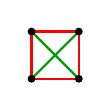
\begin{tikzpicture}[scale=0.6, baseline=(current bounding box.center)]
    \coordinate (a) at (0,1); \coordinate (b) at (1,1);
    \coordinate (c) at (1,0); \coordinate (d) at (0,0);
    
    % Red C4
    \draw[red, thick] (a)--(b)--(c)--(d)--(a);
    
    % Green diagonals
    \draw[green!60!black, thick] (a)--(c);
    \draw[green!60!black, thick] (b)--(d);
    
    \foreach \p in {a,b,c,d} \filldraw (\p) circle (2pt);
\end{tikzpicture}
\end{center}
is a colouring of $K_4$ which neither contains a red $C_3$ nor a green $P_3$.

Now consider an arbitrary edge 2-colouring of $K_5$. Pick $v_1 \in V(K_5)$ arbitrary. If two of the edges incident with $v_1$ are green, we obtain a green $P_3$. Otherwise, all but one edge must be red, say $v_1v_2, v_1v_3$ and $v_1v_4$ are red.
Following the same argument, if both of $v_2v_3$ and $v_2v_4$ are green, we obtain a green $P_3$. Otherwise, at least one, say $v_2v_3$, must be red and we obtain a red $C_3$ on $\{v_1, v_2, v_3\}$.
\begin{center}
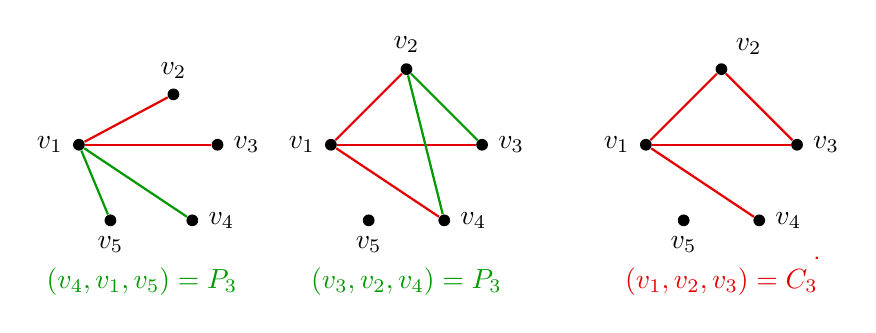
\begin{tikzpicture}[
    scale=0.8,
    dot/.style={circle, fill=black, inner sep=1.5pt},
    red_edge/.style={red!90!black, thick},
    green_edge/.style={green!60!black, thick},
    font=\sffamily
]

% --- Graph 1 (Left) ---
\begin{scope}[shift={(0,0)}]

    % Nodes
    \node[dot, label=left:$v_1$] (v1) at (0,0) {};
    \node[dot, label=above:$v_2$] (v2) at (1.5, 0.8) {};
    \node[dot, label=right:$v_3$] (v3) at (2.2, 0) {};
    \node[dot, label=right:$v_4$] (v4) at (1.8, -1.2) {};
    \node[dot, label=below:$v_5$] (v5) at (0.5, -1.2) {};

    % Edges
    \draw[red_edge] (v1) -- (v2);
    \draw[red_edge] (v1) -- (v3);
    \draw[green_edge] (v1) -- (v4);
    \draw[green_edge] (v1) -- (v5);

    % Caption
    \node[green!60!black, anchor=north] at (1, -1.8) {$(v_4, v_1, v_5) = P_3$};
\end{scope}

% --- Graph 2 (Middle) ---
\begin{scope}[shift={(5,0)}]
    % Nodes (Pentagon-ish layout)
    \node[dot, label=left:$v_1$] (v1) at (-1, 0) {};
    \node[dot, label=above:$v_2$] (v2) at (0.2, 1.2) {};
    \node[dot, label=right:$v_3$] (v3) at (1.4, 0) {};
    \node[dot, label=right:$v_4$] (v4) at (0.8, -1.2) {};
    \node[dot, label=below:$v_5$] (v5) at (-0.4, -1.2) {};

    % Edges
    % Red: v1 connects to v2, v3, v4
    \draw[red_edge] (v1) -- (v2);
    \draw[red_edge] (v1) -- (v3);
    \draw[red_edge] (v1) -- (v4);
    
    % Green: v2 connects to v3, v4
    \draw[green_edge] (v2) -- (v3);
    \draw[green_edge] (v2) -- (v4);

    % Caption
    \node[green!60!black, anchor=north] at (0.2, -1.8) {$(v_3, v_2, v_4) = P_3$};
\end{scope}

% --- Graph 3 (Right) ---
\begin{scope}[shift={(10,0)}]
    % Nodes (Same layout as middle)
    \node[dot, label=left:$v_1$] (v1) at (-1, 0) {};
    \node[dot, label=above right:$v_2$] (v2) at (0.2, 1.2) {};
    \node[dot, label=right:$v_3$] (v3) at (1.4, 0) {};
    \node[dot, label=right:$v_4$] (v4) at (0.8, -1.2) {};
    \node[dot, label=below:$v_5$] (v5) at (-0.4, -1.2) {};

    % Edges
    % Red Triangle (v1, v2, v3)
    \draw[red_edge] (v1) -- (v2);
    \draw[red_edge] (v2) -- (v3);
    \draw[red_edge] (v3) -- (v1);
    
    % Red Tail (v1 to v4)
    \draw[red_edge] (v1) -- (v4);

    % Caption
    \node[red!90!black, anchor=north] at (0.2, -1.8) {$(v_1, v_2, v_3) = C_3$};
    % Small period at the end
    \node[red!90!black, anchor=west] at (1.5, -1.8) {.};
\end{scope}

\end{tikzpicture}
\end{center}
\end{example}